\section{Computational Results}
\label{sec:results}
% Prevent result tables from floating above their section heading.
\suppressfloats[t]

The first results concern the aggregate LOS study. The room/Mesa campaign
and its separate median/oracle comparison follow in
Sections~\ref{sec:room-results} and~\ref{sec:duration-results}. Each family
retains its own objective, workloads and experimental replication unit.

\subsection{Solution quality and computation time}

Table~\ref{tab:los-legacy} retains the original five-method comparison.
For the large workload, SA, tabu and the hybrid achieve mean nominal costs
near 5198--5207, close to the overload-based lower bound. Default GA has a
mean cost of 8569.4; changing its mutation probability to $1/n$ reduces this
to 5286.9 in the sensitivity comparison. Thus, the default result does not
establish an inherent weakness of genetic search. ACO reaches 5783.5 and
requires about 10.08 seconds, compared with 0.27 for SA and 0.33 for tabu.
These runtimes are measurements from the contributor's machine and campaign,
not hardware-independent guarantees. On the small instance, all five methods
have costs around 3.25--3.29, with no session or bed overload, so the instance
provides little discrimination between them.

% Generated by scripts/summarise_los_results.py; do not edit manually.
\begin{table}[tbp]
\centering
\small
\caption{Original five-method campaign: nominal cost for the large workload (mean $\pm$ SD, ten seeds), and planning time averaged over point and upper-bound modes. GA uses its default mutation probability here; ACO was not run in the later split-session campaign.}
\label{tab:los-legacy}
\begin{tabularx}{\textwidth}{@{}Yrrr@{}}
\toprule
Method & Large cost & Small (s) & Large (s) \\
\midrule
SA & $5206.7 \pm 26.2$ & 0.11 & 0.27 \\
Tabu & $5198.4 \pm 0.0$ & 0.13 & 0.33 \\
Hybrid & $5198.3 \pm 0.0$ & 0.21 & 0.53 \\
GA (default) & $8569.4 \pm 521.3$ & 0.28 & 0.87 \\
ACO & $5783.5 \pm 170.0$ & 0.99 & 10.08 \\
\bottomrule
\end{tabularx}
\end{table}


Table~\ref{tab:los-quality} and Figure~\ref{fig:los-granularity} compare
point-LOS planning across session structures. With one 480-minute session,
tabu and the hybrid have mean gaps of about 0.16\% to the lower bound,
compared with 0.32\% for SA and 1.87\% for tuned GA. With two 240-minute
sessions, the hybrid's mean cost is 5485.9, a 5.70\% gap, compared with
5892.3 for tabu, 6022.1 for SA and 7217.0 for tuned GA. The hybrid has the
lowest mean cost among the four methods tested in that configuration; this
comparison cannot establish its superiority to the untested ACO variant.

% Generated by scripts/summarise_los_results.py; do not edit manually.
\begin{table}[tbp]
\centering
\small
\caption{Large workload: point-LOS schedule cost (mean $\pm$ SD over ten seeds), gap to the session-overload lower bound of 5190, and mean planning time. These are gaps to a lower bound, not certified gaps to the true optimum.}
\label{tab:los-quality}
\begin{tabularx}{\textwidth}{@{}Yrrr@{}}
\toprule
Method & Cost & Bound gap & Time (s) \\
\midrule
\multicolumn{4}{@{}l}{\emph{One 480-minute session per speciality-day}} \\
SA & $5206.7 \pm 26.2$ & 0.32\% & 0.276 \\
Tabu & $5198.4 \pm 0.0$ & 0.16\% & 0.336 \\
Hybrid & $5198.3 \pm 0.0$ & 0.16\% & 0.543 \\
GA ($p_{\mathrm{mut}}=1/n$) & $5286.9 \pm 44.1$ & 1.87\% & 0.793 \\
\midrule
\multicolumn{4}{@{}l}{\emph{Two 240-minute sessions per speciality-day}} \\
SA & $6022.1 \pm 196.8$ & 16.03\% & 0.385 \\
Tabu & $5892.3 \pm 347.1$ & 13.53\% & 0.441 \\
Hybrid & $5485.9 \pm 115.1$ & 5.70\% & 0.755 \\
GA ($p_{\mathrm{mut}}=1/n$) & $7217.0 \pm 333.0$ & 39.06\% & 1.176 \\
\bottomrule
\end{tabularx}
\end{table}


\begin{figure}[tbp]
\centering
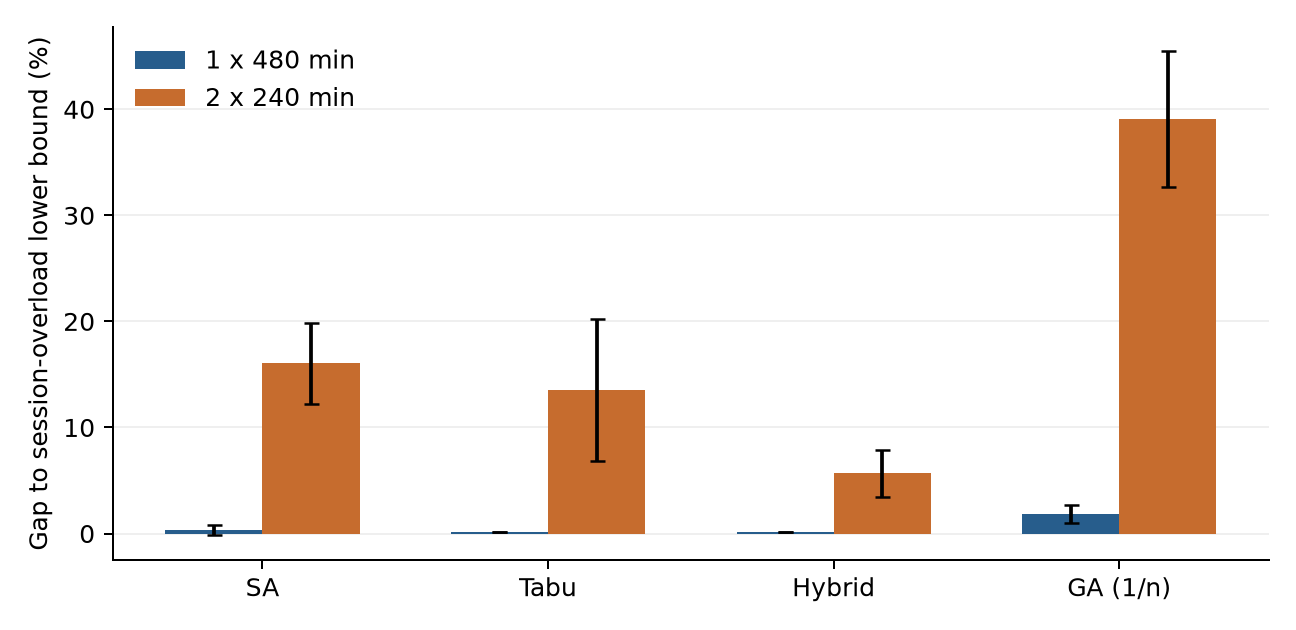
\includegraphics[width=0.88\linewidth]{figures/los-granularity.png}
\caption{Effect of session granularity on nominal schedule quality. Total
speciality-day capacity is unchanged. Bars show mean percentage gaps to the
5190 lower bound; error bars show SD across ten seeds.}
\label{fig:los-granularity}
\end{figure}

Splitting capacity changes the assignment landscape even though the total
number of available minutes is unchanged. The observed ranking therefore
depends on session granularity as well as the algorithm. The hybrid also
uses more computation: its mean point-planning runtime in the split-session
campaign is 0.755 seconds, versus 0.385 for SA and 0.441 for tabu. This is an instance-specific comparison under unequal computation;
the lower-bound gap does not prove optimality.

\subsection{LOS scenarios and upper-bound planning}

For the large workload, mean rounded nominal LOS is about 1.90 days. The
floor-noise scenarios average about 2.10 days, while the alternative symmetric
rule averages about 1.98 days. Clipping and differences between unrounded
predictions and rounded nominal inputs therefore change the mean as well
as variability. Under point planning, the original floor-noise evaluation
raises expected cost by about 109--115 for SA, tabu and the hybrid. Since
only LOS changes when a schedule is re-evaluated, this increase acts through
the bed term of Equation~\ref{eq:los-cost}; it is not deterioration in room
assignment itself.

The effect of upper-bound planning is best assessed using paired expected
costs rather than the increase relative to each schedule's own nominal
baseline. Table~\ref{tab:los-robustness} and
Figure~\ref{fig:los-uncertainty} retain the configuration and scenario labels
for this comparison. In the one-session configuration, upper-bound planning
increases scenario-mean cost by 68.4 for SA, 63.1 for tabu and 102.3 for the
hybrid. The source also reports lower dispersion, indicating a cost/predictability
trade-off.

% Generated by scripts/summarise_los_results.py; do not edit manually.
\begin{table}[tbp]
\centering
\small
\caption{Paired change in scenario-mean cost, upper-bound planning minus point planning (mean $\pm$ SE across ten seeds). Negative values favour upper-bound planning. Floor-noise scenarios and horizon-truncated bed tracking are used in both configurations.}
\label{tab:los-robustness}
\begin{tabularx}{\textwidth}{@{}Yrr@{}}
\toprule
Method & $1\times480$ min & $2\times240$ min \\
\midrule
SA & $+68.4 \pm 12.0$ & $-88.6 \pm 68.8$ \\
Tabu & $+63.1 \pm 12.9$ & $+31.3 \pm 87.6$ \\
Hybrid & $+102.3 \pm 7.9$ & $+9.1 \pm 34.1$ \\
GA ($p_{\mathrm{mut}}=1/n$) & $-12.0 \pm 19.6$ & $-98.4 \pm 167.8$ \\
\bottomrule
\end{tabularx}
\end{table}


\begin{figure}[tbp]
\centering
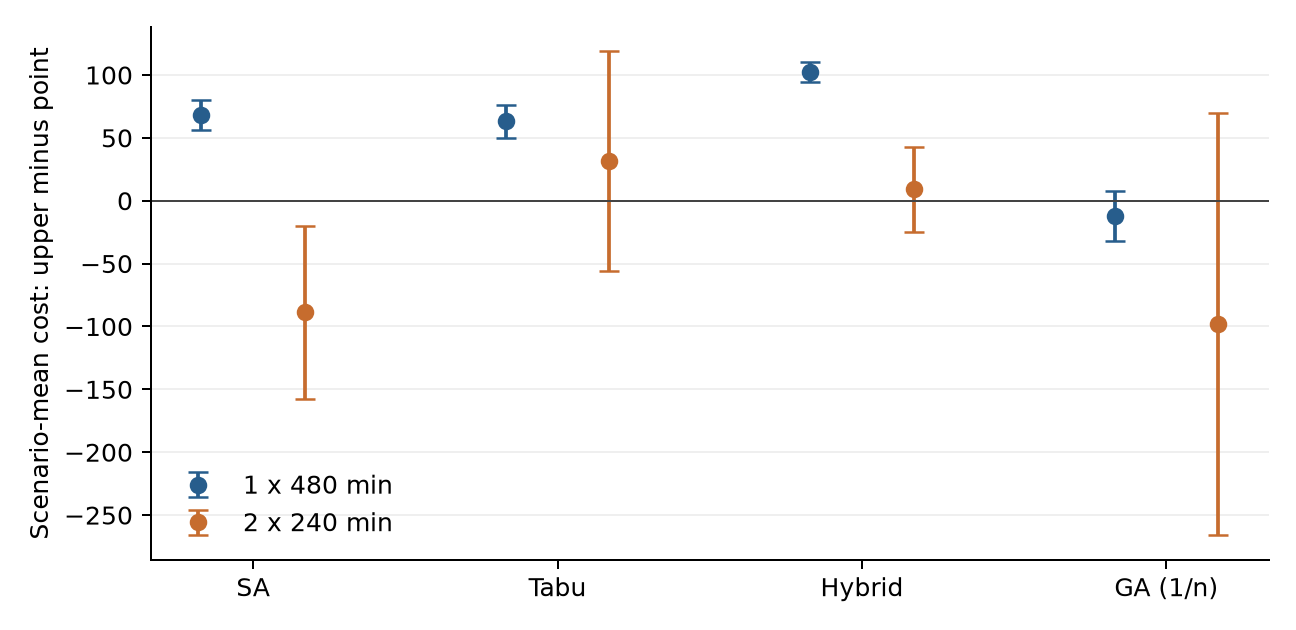
\includegraphics[width=0.88\linewidth]{figures/los-uncertainty.png}
\caption{Paired scenario-mean cost differences for upper-bound versus point
planning, using floor noise and horizon-truncated bed accounting. Error bars
are one SE across ten paired seeds, not confidence intervals. Negative values
favour upper-bound planning.}
\label{fig:los-uncertainty}
\end{figure}

The two-session results are less conclusive: paired differences are
$-88.6\pm68.8$ for SA, $31.3\pm87.6$ for tabu, $9.1\pm34.1$ for the hybrid
and $-98.4\pm167.8$ for tuned GA, expressed as mean $\pm$ SE. These results show a method-dependent effect with substantial uncertainty;
a uniform increase or benefit under this configuration is not established. More generally, a
small increase from a schedule's own baseline is not evidence of lower
absolute cost or protection from extreme failures. Scenario distributions,
horizon treatment and the cost baseline must remain explicit.

\subsection{Load, matching and horizon sensitivity}

Figure~\ref{fig:los-load} preserves the source study's load experiment with
an explicit axis definition. The varied quantity is operating-block load
for the bottleneck speciality, obtained by changing session capacity; the
figure does not establish a critical bed-utilisation threshold at 93\%.
The bed capacity is fixed and only four target block loads are examined.
Five seeds per load also limit the precision of comparisons.

\begin{figure}[tbp]
\centering
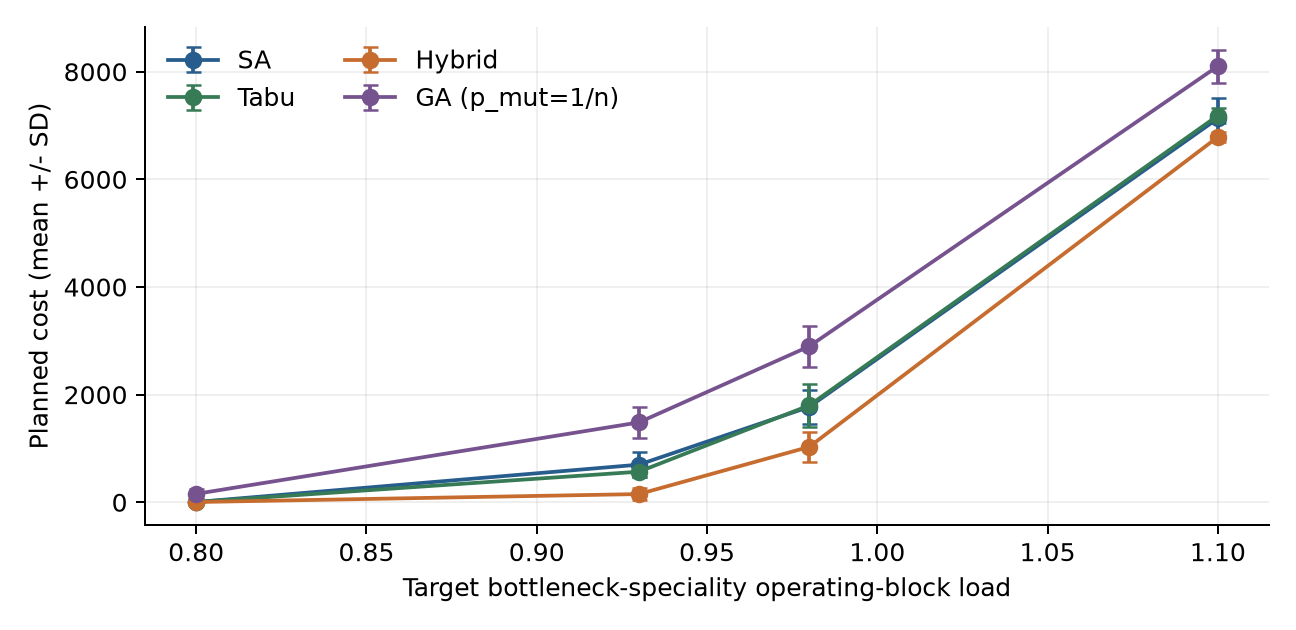
\includegraphics[width=0.88\linewidth]{figures/los-block-load.png}
\caption{Planned cost versus target operating-block load for the two-session
configuration. Points show means and error bars show SD over five seeds.
The horizontal axis is not measured bed utilisation.}
\label{fig:los-load}
\end{figure}

In the matched-only workload, the overload lower bound is zero. The hybrid
achieves zero session overload and a mean nominal cost of 7.13, consisting
of workload imbalance; tabu's mean cost is 7.65. Percentages relative to a
zero lower bound are undefined. Removing 57 cases changes demand as well
as prediction matching, so the improvement cannot be attributed solely to
better model linkage. The source also examines full-stay accounting because
horizon truncation can favour postponing patients towards the last days.
Extended accounting is a sensitivity analysis of frozen plans, not a claim
that the planning objective itself has been replaced.


% Finish the LOS floats before the room-study results.
\FloatBarrier
\subsection{Room allocation: exact reference and predicted search quality}
\label{sec:room-results}

The room fixture has seven predicted durations of 30--90 minutes in ten-minute
increments, two rooms and $2^7=128$ allocations. Enumeration gives $U=0$,
$O=165$ and $C_{\mathrm{room}}=0.313688$. Table~\ref{tab:room-exact} shows
that all five searches reach this optimum at every tested seed; the greedy
baseline has an absolute cost gap of 0.80038. This is a predicted allocation certificate only: without closure, hidden
durations leave mean completions at 5.67--6 of seven cases across methods.

\begin{table}[H]
\centering\small
\caption{Small room-allocation reference: absolute initial predicted-cost gaps, exact hits and mean initial solve time. Three seeds on one fixed seven-case fixture; baseline repeats are identical.}
\label{tab:room-exact}
\begin{tabular}{@{}lrrrr@{}}
\toprule
Method & Mean gap & Worst gap & Exact hits & Time (s) \\
\midrule
Baseline & 0.80038 & 0.80038 & 0/3 & 0.000 \\
SA & 0.00000 & 0.00000 & 3/3 & 0.523 \\
Tabu & 0.00000 & 0.00000 & 3/3 & 0.521 \\
GA & 0.00000 & 0.00000 & 3/3 & 0.523 \\
Hybrid & 0.00000 & 0.00000 & 3/3 & 0.538 \\
ACO & 0.00000 & 0.00000 & 3/3 & 0.574 \\
\bottomrule
\end{tabular}
\end{table}


Table~\ref{tab:room-initial} separates predicted initial quality from execution.
At 100 cases, SA, tabu and the hybrid reduce mean predicted overtime from
668.0 minutes for the baseline to 602.0. At 300 cases, tabu and the hybrid
reach 1905.5 versus 2195.0 for the baseline; SA reaches 1908.0. All retain
zero predicted unstarted cases. GA retains the incumbent at both sizes;
ACO improves it at 100 cases but not at 300. These rankings are specific to the tested budget.

\begin{table}[H]
\centering\small
\caption{Generated workloads: initial predicted unstarted count U, overtime OT and end-to-end solve time, averaged over six plans per method and size. These predicted quantities are distinct from execution outcomes. The 300-case campaign used four concurrent batches.}
\label{tab:room-initial}
\begin{tabular}{@{}rlrrr@{}}
\toprule
Cases & Method & Predicted U & Predicted OT & Time (s) \\
\midrule
100 & Baseline & 0.00 & 668.0 & 0.002 \\
100 & SA & 0.00 & 602.0 & 0.696 \\
100 & Tabu & 0.00 & 602.0 & 0.679 \\
100 & GA & 0.00 & 668.0 & 0.697 \\
100 & Hybrid & 0.00 & 602.0 & 0.682 \\
100 & ACO & 0.00 & 616.2 & 1.366 \\
300 & Baseline & 0.00 & 2195.0 & 0.009 \\
300 & SA & 0.00 & 1908.0 & 1.098 \\
300 & Tabu & 0.00 & 1905.5 & 1.107 \\
300 & GA & 0.00 & 2195.0 & 1.128 \\
300 & Hybrid & 0.00 & 1905.5 & 1.089 \\
300 & ACO & 0.00 & 2195.0 & 3.707 \\
\bottomrule
\end{tabular}
\end{table}


The mean initial time is approximately 0.68--0.70 seconds for the four
non-ACO searches at 100 cases, compared with 1.37 seconds for ACO. At
300 cases, corresponding means are approximately 1.09--1.13 and 3.71 seconds.
Baseline timing excludes a search worker. Per-candidate work differs, and
concurrent 300-case execution limits cross-size timing interpretation. Larger
room instances have no certified optimum or optimality gap.

\subsection{Static and reactive execution under room closure}

Historical outcomes vary by day (Table~\ref{tab:room-historical}). All methods
complete nine cases on 3 January under both policies, but reactive overtime
is higher. On 2 February, tabu and the hybrid move from 12.00 completed cases
and 158.7 overtime minutes under static execution to 11.33 and 108.0 under
reactive execution. Lower overtime here accompanies fewer completed cases.
On 20 October, all methods complete 16 of 25 cases under both policies, while
reactive overtime falls from 110 minutes to about 73.7--82.7. Day-level comparisons therefore matter.

\begin{table}[H]
\centering\small
\caption{Historical closure scenario: mean completed cases and realised overtime over three solver seeds per day. S = static; R = reactive. Each pair shares its initial plan. Overtime includes turnover and sums minutes over rooms.}
\label{tab:room-historical}
\begin{tabular}{@{}llrrrr@{}}
\toprule
Date & Method & Done S & Done R & OT S & OT R \\
\midrule
2022-01-03 & Baseline & 9.00 & 9.00 & 64.0 & 92.0 \\
2022-01-03 & SA & 9.00 & 9.00 & 7.3 & 44.7 \\
2022-01-03 & Tabu & 9.00 & 9.00 & 15.7 & 57.3 \\
2022-01-03 & GA & 9.00 & 9.00 & 61.0 & 95.0 \\
2022-01-03 & Hybrid & 9.00 & 9.00 & 15.7 & 57.3 \\
2022-01-03 & ACO & 9.00 & 9.00 & 10.3 & 41.0 \\
2022-02-02 & Baseline & 11.00 & 11.00 & 59.0 & 113.0 \\
2022-02-02 & SA & 11.67 & 11.33 & 135.3 & 109.3 \\
2022-02-02 & Tabu & 12.00 & 11.33 & 158.7 & 108.0 \\
2022-02-02 & GA & 11.67 & 11.00 & 115.0 & 68.0 \\
2022-02-02 & Hybrid & 12.00 & 11.33 & 158.7 & 108.0 \\
2022-02-02 & ACO & 11.67 & 11.33 & 154.7 & 121.3 \\
2022-10-20 & Baseline & 16.00 & 16.00 & 110.0 & 77.0 \\
2022-10-20 & SA & 16.00 & 16.00 & 110.0 & 74.0 \\
2022-10-20 & Tabu & 16.00 & 16.00 & 110.0 & 75.7 \\
2022-10-20 & GA & 16.00 & 16.00 & 110.0 & 73.7 \\
2022-10-20 & Hybrid & 16.00 & 16.00 & 110.0 & 75.7 \\
2022-10-20 & ACO & 16.00 & 16.00 & 110.0 & 82.7 \\
\bottomrule
\end{tabular}
\end{table}


The generated closure workloads also show mixed effects
(Table~\ref{tab:room-generated}). At 300 cases, baseline replanning raises
mean completions from 287.5 to 289.5 and overtime from 2838.0 to 3319.5
room-minutes. Tabu and the hybrid begin at 289.0 completions under static
execution and fall to 287.33 and 287.50 respectively when reactive. These
policy differences are conditional on each method's shared initial plan;
they do not compare methods from a common initial allocation.

\begin{table}[H]
\centering\small
\caption{Generated closure scenario: means over two sampled workloads and three solver seeds (six runs per cell). Resources are 14/15 rooms for 100 cases and 44/45 for 300 cases. OT is realised overtime including turnover, in room-minutes.}
\label{tab:room-generated}
\begin{tabular}{@{}rlrrrr@{}}
\toprule
Cases & Method & Done S & Done R & OT S & OT R \\
\midrule
100 & Baseline & 97.00 & 97.00 & 933.5 & 1022.0 \\
100 & SA & 96.67 & 96.17 & 952.5 & 958.5 \\
100 & Tabu & 96.50 & 95.67 & 876.0 & 856.0 \\
100 & GA & 97.00 & 96.33 & 933.5 & 971.7 \\
100 & Hybrid & 96.50 & 96.17 & 876.0 & 932.8 \\
100 & ACO & 96.33 & 96.00 & 902.5 & 976.0 \\
300 & Baseline & 287.50 & 289.50 & 2838.0 & 3319.5 \\
300 & SA & 287.33 & 286.33 & 2923.0 & 3028.5 \\
300 & Tabu & 289.00 & 287.33 & 3021.5 & 3140.5 \\
300 & GA & 287.50 & 286.00 & 2838.0 & 2974.5 \\
300 & Hybrid & 289.00 & 287.50 & 3021.5 & 3165.5 \\
300 & ACO & 287.50 & 285.17 & 2838.0 & 3000.5 \\
\bottomrule
\end{tabular}
\end{table}


Across all 144 closure pairs, reactive execution completes more cases in 16,
the same number in 83 and fewer in 45. Overtime falls in 64, ties in seven
and rises in 73. The counts include deterministic baseline repeats and are descriptive.
All no-closure static/reactive pairs have identical completion, overtime,
occupancy and total delay, as expected when no replanning trigger occurs.

\begin{figure}[H]
\centering
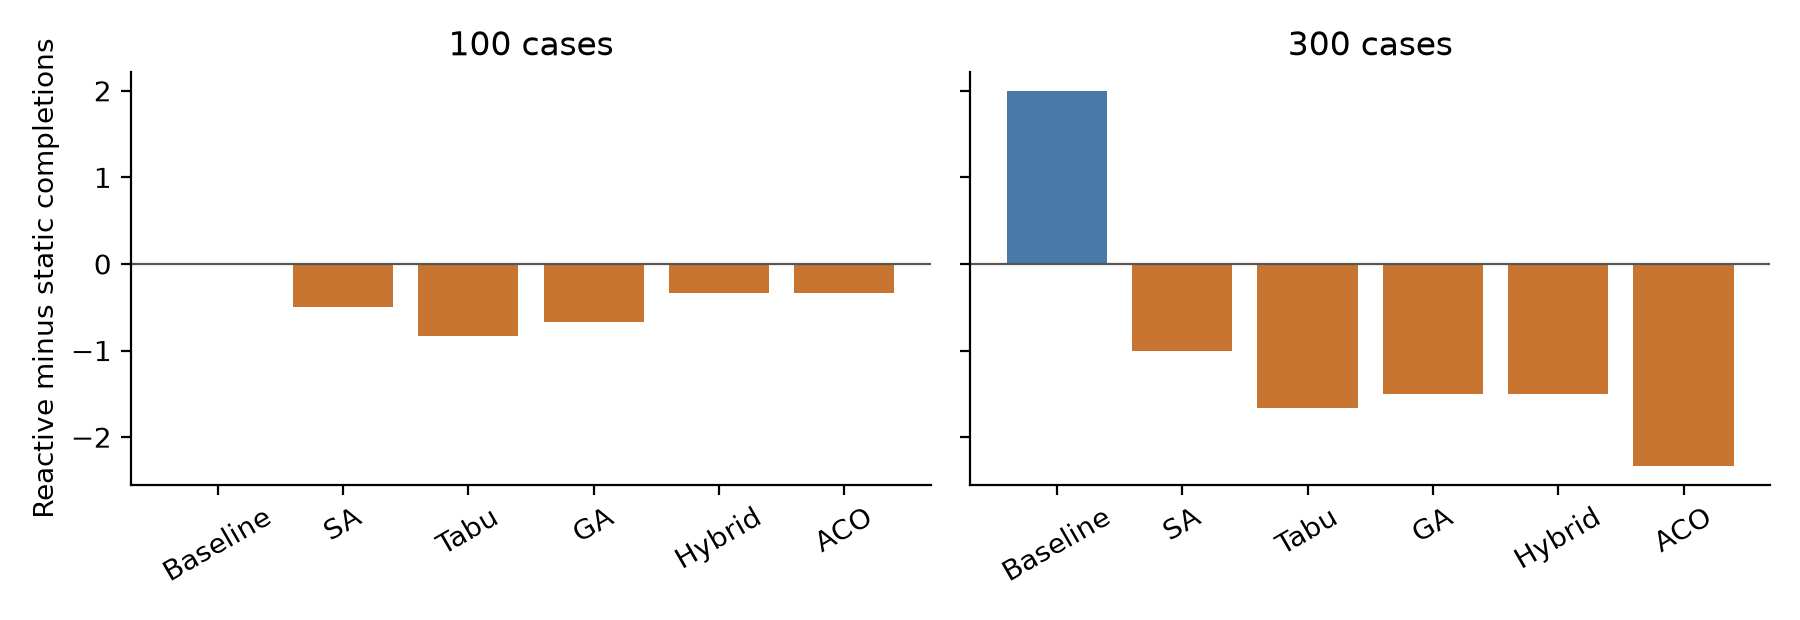
\includegraphics[width=0.95\linewidth]{figures/room-policy-differences.png}
\caption{Mean paired completion differences under closure in the primary
room campaign. Each bar averages two generated workloads and three solver
seeds; positive values favour reactive execution. No confidence intervals
or statistical superiority are claimed. Read alongside overtime in
Table~\ref{tab:room-generated}.}
\label{fig:room-policy}
\end{figure}

\subsection{Perfect duration information: a separate execution comparison}
\label{sec:duration-results}

Table~\ref{tab:room-duration} uses the separate median/oracle campaign,
restricting the displayed comparison to no-closure static execution so
neither disruption nor reactive replanning changes between modes. At 300
cases, oracle estimates allow all six methods to complete 300 cases on average,
compared with 287.5--289.17 under median estimates. Oracle overtime is
3590.5--3678.0 room-minutes, compared with 2779.0--2965.0: additional throughput
comes with more post-closing occupancy, consistent with the objective's
priority for case starts.

\begin{table}[H]
\centering\small
\caption{Separate duration-information campaign: no-closure static execution. M = historical-median estimates; O = oracle durations. Means use two workloads and three solver seeds. Resources and hidden outcomes are held fixed across modes; initial plans are recomputed. OT includes turnover.}
\label{tab:room-duration}
\begin{tabular}{@{}rlrrrr@{}}
\toprule
Cases & Method & Done M & Done O & OT M & OT O \\
\midrule
100 & Baseline & 97.50 & 99.50 & 922.0 & 886.0 \\
100 & SA & 97.17 & 100.00 & 942.7 & 908.5 \\
100 & Tabu & 97.17 & 100.00 & 874.7 & 908.5 \\
100 & GA & 97.50 & 99.50 & 922.0 & 883.3 \\
100 & Hybrid & 97.17 & 100.00 & 874.7 & 908.5 \\
100 & ACO & 97.17 & 100.00 & 908.5 & 927.5 \\
300 & Baseline & 287.50 & 300.00 & 2779.0 & 3678.0 \\
300 & SA & 288.00 & 300.00 & 2949.7 & 3590.5 \\
300 & Tabu & 289.17 & 300.00 & 2965.0 & 3590.5 \\
300 & GA & 287.50 & 300.00 & 2779.0 & 3678.0 \\
300 & Hybrid & 289.17 & 300.00 & 2965.0 & 3590.5 \\
300 & ACO & 287.50 & 300.00 & 2779.0 & 3678.0 \\
\bottomrule
\end{tabular}
\end{table}


At 100 cases, the four non-GA searches complete all 100 cases under oracle
estimates, whereas baseline and GA complete 99.5 on average. In the small
fixture, each metaheuristic completes all seven cases with 240 overtime
minutes under oracle information; the baseline still completes six with
105 minutes. Perfect information therefore does not compensate for every
search or representation restriction, nor does it necessarily lower overtime.
Duration substitution also changes ordering and search landscape. Learned
models require their own held-out end-to-end comparison; oracle gains do
not estimate their operational benefit.

